% Options for packages loaded elsewhere
\PassOptionsToPackage{unicode}{hyperref}
\PassOptionsToPackage{hyphens}{url}
%
\documentclass[
]{book}
\usepackage{lmodern}
\usepackage{amssymb,amsmath}
\usepackage{ifxetex,ifluatex}
\ifnum 0\ifxetex 1\fi\ifluatex 1\fi=0 % if pdftex
  \usepackage[T1]{fontenc}
  \usepackage[utf8]{inputenc}
  \usepackage{textcomp} % provide euro and other symbols
\else % if luatex or xetex
  \usepackage{unicode-math}
  \defaultfontfeatures{Scale=MatchLowercase}
  \defaultfontfeatures[\rmfamily]{Ligatures=TeX,Scale=1}
\fi
% Use upquote if available, for straight quotes in verbatim environments
\IfFileExists{upquote.sty}{\usepackage{upquote}}{}
\IfFileExists{microtype.sty}{% use microtype if available
  \usepackage[]{microtype}
  \UseMicrotypeSet[protrusion]{basicmath} % disable protrusion for tt fonts
}{}
\makeatletter
\@ifundefined{KOMAClassName}{% if non-KOMA class
  \IfFileExists{parskip.sty}{%
    \usepackage{parskip}
  }{% else
    \setlength{\parindent}{0pt}
    \setlength{\parskip}{6pt plus 2pt minus 1pt}}
}{% if KOMA class
  \KOMAoptions{parskip=half}}
\makeatother
\usepackage{xcolor}
\IfFileExists{xurl.sty}{\usepackage{xurl}}{} % add URL line breaks if available
\IfFileExists{bookmark.sty}{\usepackage{bookmark}}{\usepackage{hyperref}}
\hypersetup{
  pdftitle={Introdução ao R Markdown},
  pdfauthor={Eduardo José de Campos Lemos Júnior, Samuel Vianna Quintanilha},
  hidelinks,
  pdfcreator={LaTeX via pandoc}}
\urlstyle{same} % disable monospaced font for URLs
\usepackage{color}
\usepackage{fancyvrb}
\newcommand{\VerbBar}{|}
\newcommand{\VERB}{\Verb[commandchars=\\\{\}]}
\DefineVerbatimEnvironment{Highlighting}{Verbatim}{commandchars=\\\{\}}
% Add ',fontsize=\small' for more characters per line
\usepackage{framed}
\definecolor{shadecolor}{RGB}{248,248,248}
\newenvironment{Shaded}{\begin{snugshade}}{\end{snugshade}}
\newcommand{\AlertTok}[1]{\textcolor[rgb]{0.94,0.16,0.16}{#1}}
\newcommand{\AnnotationTok}[1]{\textcolor[rgb]{0.56,0.35,0.01}{\textbf{\textit{#1}}}}
\newcommand{\AttributeTok}[1]{\textcolor[rgb]{0.77,0.63,0.00}{#1}}
\newcommand{\BaseNTok}[1]{\textcolor[rgb]{0.00,0.00,0.81}{#1}}
\newcommand{\BuiltInTok}[1]{#1}
\newcommand{\CharTok}[1]{\textcolor[rgb]{0.31,0.60,0.02}{#1}}
\newcommand{\CommentTok}[1]{\textcolor[rgb]{0.56,0.35,0.01}{\textit{#1}}}
\newcommand{\CommentVarTok}[1]{\textcolor[rgb]{0.56,0.35,0.01}{\textbf{\textit{#1}}}}
\newcommand{\ConstantTok}[1]{\textcolor[rgb]{0.00,0.00,0.00}{#1}}
\newcommand{\ControlFlowTok}[1]{\textcolor[rgb]{0.13,0.29,0.53}{\textbf{#1}}}
\newcommand{\DataTypeTok}[1]{\textcolor[rgb]{0.13,0.29,0.53}{#1}}
\newcommand{\DecValTok}[1]{\textcolor[rgb]{0.00,0.00,0.81}{#1}}
\newcommand{\DocumentationTok}[1]{\textcolor[rgb]{0.56,0.35,0.01}{\textbf{\textit{#1}}}}
\newcommand{\ErrorTok}[1]{\textcolor[rgb]{0.64,0.00,0.00}{\textbf{#1}}}
\newcommand{\ExtensionTok}[1]{#1}
\newcommand{\FloatTok}[1]{\textcolor[rgb]{0.00,0.00,0.81}{#1}}
\newcommand{\FunctionTok}[1]{\textcolor[rgb]{0.00,0.00,0.00}{#1}}
\newcommand{\ImportTok}[1]{#1}
\newcommand{\InformationTok}[1]{\textcolor[rgb]{0.56,0.35,0.01}{\textbf{\textit{#1}}}}
\newcommand{\KeywordTok}[1]{\textcolor[rgb]{0.13,0.29,0.53}{\textbf{#1}}}
\newcommand{\NormalTok}[1]{#1}
\newcommand{\OperatorTok}[1]{\textcolor[rgb]{0.81,0.36,0.00}{\textbf{#1}}}
\newcommand{\OtherTok}[1]{\textcolor[rgb]{0.56,0.35,0.01}{#1}}
\newcommand{\PreprocessorTok}[1]{\textcolor[rgb]{0.56,0.35,0.01}{\textit{#1}}}
\newcommand{\RegionMarkerTok}[1]{#1}
\newcommand{\SpecialCharTok}[1]{\textcolor[rgb]{0.00,0.00,0.00}{#1}}
\newcommand{\SpecialStringTok}[1]{\textcolor[rgb]{0.31,0.60,0.02}{#1}}
\newcommand{\StringTok}[1]{\textcolor[rgb]{0.31,0.60,0.02}{#1}}
\newcommand{\VariableTok}[1]{\textcolor[rgb]{0.00,0.00,0.00}{#1}}
\newcommand{\VerbatimStringTok}[1]{\textcolor[rgb]{0.31,0.60,0.02}{#1}}
\newcommand{\WarningTok}[1]{\textcolor[rgb]{0.56,0.35,0.01}{\textbf{\textit{#1}}}}
\usepackage{longtable,booktabs}
% Correct order of tables after \paragraph or \subparagraph
\usepackage{etoolbox}
\makeatletter
\patchcmd\longtable{\par}{\if@noskipsec\mbox{}\fi\par}{}{}
\makeatother
% Allow footnotes in longtable head/foot
\IfFileExists{footnotehyper.sty}{\usepackage{footnotehyper}}{\usepackage{footnote}}
\makesavenoteenv{longtable}
\usepackage{graphicx}
\makeatletter
\def\maxwidth{\ifdim\Gin@nat@width>\linewidth\linewidth\else\Gin@nat@width\fi}
\def\maxheight{\ifdim\Gin@nat@height>\textheight\textheight\else\Gin@nat@height\fi}
\makeatother
% Scale images if necessary, so that they will not overflow the page
% margins by default, and it is still possible to overwrite the defaults
% using explicit options in \includegraphics[width, height, ...]{}
\setkeys{Gin}{width=\maxwidth,height=\maxheight,keepaspectratio}
% Set default figure placement to htbp
\makeatletter
\def\fps@figure{htbp}
\makeatother
\usepackage[normalem]{ulem}
% Avoid problems with \sout in headers with hyperref
\pdfstringdefDisableCommands{\renewcommand{\sout}{}}
\setlength{\emergencystretch}{3em} % prevent overfull lines
\providecommand{\tightlist}{%
  \setlength{\itemsep}{0pt}\setlength{\parskip}{0pt}}
\setcounter{secnumdepth}{5}

\title{Introdução ao R Markdown}
\author{Eduardo José de Campos Lemos Júnior, Samuel Vianna Quintanilha}
\date{2020-08-05}

\begin{document}
\maketitle

{
\setcounter{tocdepth}{1}
\tableofcontents
}
\hypertarget{intro}{%
\chapter{Introdção}\label{intro}}

Neste curso, iremos aprender a utilizar o R Markdown para gerar documentos.
\#\# O que é
Markdown é uma linguagem de marcação usada para formatar de maneira simples os textos redigidos e converte-los em HTML. John Gruber e Aaron Swartz, os criadores desse sistema, utilizaram marcadores como: \#, * ,! , {[}{]} e (). Assim é possível inserir em nossos textos: títulos, listas, formatação de fonte, imagens e tabelas.
R Markdown é um documento criado no R Studio (Ou em outras IDEs) que possibilita empregar os recursos da linguagem markdown citados acima em conjunto com a linguagem R, permitindo a melhor organização de análises, relatórios e códigos em um só documento.

\hypertarget{possuxedveis-tipos-de-outputs}{%
\section{Possíveis tipos de Outputs}\label{possuxedveis-tipos-de-outputs}}

O R Markdown apresenta várias possibilidades de outputs (renderizar) nos formatos de documentos, apresentações, entre outros, sendo que em cada formato há várias opções de customização. Vejamos abaixo os principais:
Documentos
-html\_document -- documento no formato HTML;
-pdf\_document -- documento no formato PDF (via o modelo LaTeX);
-word\_document -- documento no formato do editor de texto Microsoft Word (docx);
-odt\_documento -- documento no formato dos editores de texto Libre Office e OpenDocument;
-rtf\_documento -- documento no formato Rich Text Format (rtf).

Apresentações (slides)
-ioslides\_presentation -- apresentação no formato HTML com ioslides;
-beamer\_presentation -- apresentação no formato PDF com LaTeX Beamer;
-powerpoint\_presentation -- apresentação no formato power point.

Outros
-flexdashboard::flex\_dashboard -- apresentação interativa com dashboards;
-htm\_vignette -- R package vignette no format HTML
-github\_document -- document no format GitHub

Você pode escolher o output desejado quando for criar um documento conforme a figura 1. Para fazer deve-se clicar em file \textgreater{} new file \textgreater{} R Markdown. Abrirá uma aba e nela há quatro formas de output previamente estabelecidas, a saber: Document (HTML, PDF e Word), Presentation (HTML (ioslides), HTML (slidy), PDF (Beamer) e PowerPoint), Shiny (Shiny Document e Shy Presentation) e From Template (GitHub document e Package Vignette). Escolha uma e clique em OK.
Além disso, você também pode alterar o formato utilizando a função abaixo, sendo que render refere-se ao local que está salvo seu documento e output\_format ao tipo de documento desejado, conforme os exemplos apontados no início.

\texttt{render("teste.Rmd",\ output\_format\ =\ "pdf\_document")}

O mesmo pode ser feito para outros formatos.

\begin{itemize}
\tightlist
\item
  \texttt{beamer\_presentation}
\item
  \texttt{context\_document}
\item
  \texttt{github\_document}
\item
  \texttt{html\_document}
\item
  \texttt{ioslides\_presentation}
\item
  \texttt{latex\_document}
\item
  \texttt{md\_document}
\item
  \texttt{odt\_document}
\item
  \texttt{pdf\_document}
\item
  \texttt{powerpoint\_presentation}
\item
  \texttt{rtf\_document}
\item
  \texttt{slidy\_presentation}
\item
  \texttt{word\_document}
\end{itemize}

\hypertarget{download-rmd-e-latex}{%
\section{Download (rmd e latex)}\label{download-rmd-e-latex}}

Para exportar um arquivo PDF utilizando o R Markdown é necessário um motor LaTex pois é ele que irá converter o arquivo .tex em PDF.
Então é necessário que tenha instalado em seu computador a \emph{(biblioteca?)} MiKTeX,. Para fazer o download é só acessar o link: \url{https://miktex.org/download}.

\hypertarget{windows}{%
\subsection{Windows}\label{windows}}

Selecione a aba Windows e clique no botão de download:

\includegraphics{download_MiKTex/download_windowns_MiKTex.png}
\#\#\# Linux
Selecione a aba Linux em seguida a aba de sua distribuição Linux para receber as instruções de instalação:

\includegraphics{download_MiKTex/download_linux_MiKTex.png}
\#\#\# MacOS
Selecione a aba macOS e clique no botão de download:

\includegraphics{download_MiKTex/download_macOS_MiKTex.png}
\#\# Criando o primeiro documento
Para gerar um arquivo em R Markdown é necessário abrir o programa R Studio, e instalar o pacote rmarkdown :

\includegraphics{Imagem/ins.png}
Após a instalação do pacote no R Studio, siga os seguintes passos:
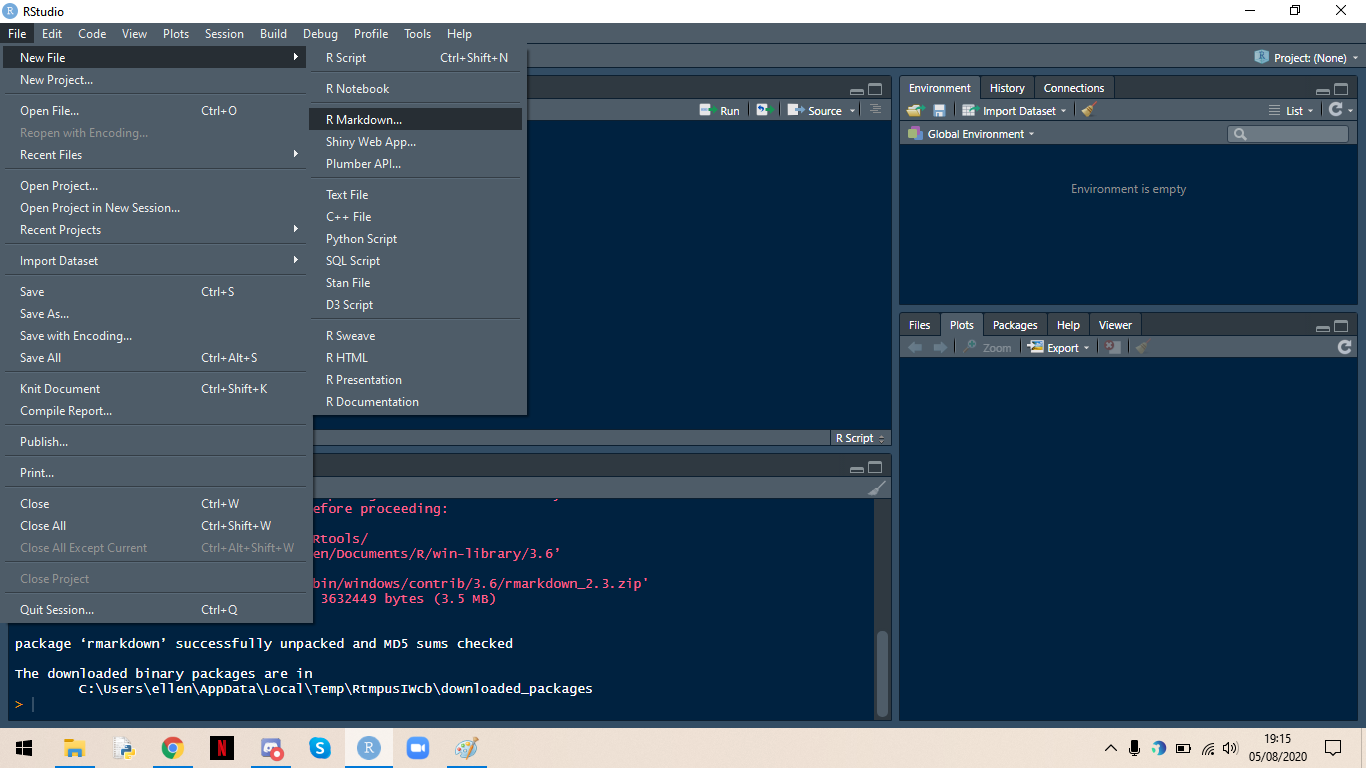
\includegraphics{Imagem/new.png}
- Em seguida, escolha o tipo de arquivo desejado:

\includegraphics{Imagem/file.png}
Obs: Para gerar documentos em PDF, é necessário ter instalado em seu computador o programa \href{https://miktex.org/}{Latex}

Seguindo os passos acima, você terá criado o seu primeiro documento em R Markdown.

Vale ressaltar que é possível utilizar o R Markdown sem que tenha instalado o R Studio, porém, é necessário ter instalado o programa \href{https://pandoc.org}{Pandoc}

\begin{verbatim}

```r
print(2)
```

```
## [1] 2
```

\end{verbatim}

\hypertarget{sintaxe}{%
\chapter{Sintaxe}\label{sintaxe}}

\hypertarget{pruxeaambulo}{%
\section{Prêambulo}\label{pruxeaambulo}}

No início de um documento R Markdown, é utilizada a linguagem \href{https://pt.wikipedia.org/wiki/YAML}{yaml} para definir as configurações do seu arquivo.
As configurações disponiveis no preâmbulo do seu documento R Markdown são variadas, podendo inclusive ter diferentes opções para diferentes tipos de arquivos.
Uma das configurações mais importantes para se definir no seu preambulo é o \protect\hyperlink{possuxedveis-tipos-de-outputs}{tipo de documento} a ser gerado.

\hypertarget{definindo-tipo-de-output}{%
\subsection{Definindo tipo de output}\label{definindo-tipo-de-output}}

A opçao de \protect\hyperlink{possuxedveis-tipos-de-outputs}{tipo de documento} é definida da seguinte forma:

\begin{verbatim}
---
output: pdf_document
---
\end{verbatim}

No código acima, \texttt{output} foi definido como \texttt{pdf\_document()}. Output é o formato final do seu documento, e \texttt{pdf\_document()} é, dentro do pacote \texttt{rmarkdown}, o formato pdf. Para gerar arquivos de formatos diferentes, é necessário somente que seja modificado a opção de \texttt{output} no preâmbulo.
Note que a opção definida no preâmbulo foi escrita entre duas linhas tracejadas, não é possível definir suas configurações fora dessas linhas tracejadas, da mesma forma, não é possível escrever partes do seu documento ou rodar códigos de \texttt{R} dentro das linhas.
Por padrão no \texttt{yaml} utilizado no preâmbulo de R Markdown, a opção a ser definida é escrita sem espaços, seguida de dois pontos, espaço e então a definição da opção.
Existem opções dentro de outras opções, como por exemplo \texttt{pdf\_document()}, podemos definir configurações se o documento terá ou não sumário, quantos níveis de \protect\hyperlink{cabeuxe7alhos}{cabeçalho} serão utilizados no sumário, etc.

\begin{verbatim}
---
output: pdf_document:
  toc: true
  toc_depth: 3
  latex_engine: xelatex
---
\end{verbatim}

No exemplo acima, definimos \texttt{toc} (table of contents) como \texttt{true}, o que vai fazer com que seja gerado um sumário no documento final, perceba que em \texttt{yaml} o valor lógico de verdadeiro é escrito com todas as letras minúsculas. Definindo \texttt{toc\_depth} como \texttt{3}, quando o sumário for gerado, até três níveis de \protect\hyperlink{cabeuxe7alhos}{cabeçalho} apareceram no sumário.

\hypertarget{informauxe7uxf5es-gerais}{%
\subsection{Informações Gerais}\label{informauxe7uxf5es-gerais}}

Além do tipo de documento, e das opções de cada tipo de documento, podemos definir algumas opções gerais, como autor, título do documento, e data.

\begin{verbatim}
---
author: "Fulano"
output: pdf_document:
  toc: true
  toc_depth: 3
  latex_engine: xelatex
---
\end{verbatim}

Seguindo com o preâmbulo já feito anteriormente, foi adicionada a opção \texttt{author}, que irá definir o autor do seu documento. Por padrão, o autor irá aparecer na página inicial de diversos \protect\hyperlink{possuxedveis-tipos-de-outputs}{tipos de documento}.

\begin{verbatim}
---
date: 1 de janeiro de 1970
output: pdf_document:
  toc: true
  toc_depth: 3
  latex_engine: xelatex
author: Fulano
---
\end{verbatim}

Utilizando a opção \texttt{date} podemos definir uma data para o documento, semelhante ao autor, a data aparece por padrão no início dos documentos.
Perceba que no exemplo acima, o nome do autor e a data foram escritas sem aspas, mas irão funcionar da mesma forma, perceba também que a opção do autor foi trocada de ordem, as opções do preâmbulo não necessitam de uma ordem específica, mas as opções de dentro de outras opções devem sempre estar abaixo da opção mae (sei la como chamar isso) e com uma identação a mais.

\begin{verbatim}
---
author: Fulano
date: 1 de janeiro de 1970
title: Título
output: pdf_document:
  toc: true
  toc_depth: 3
  latex_engine: xelatex
---
\end{verbatim}

Por fim foi definida também a opção \texttt{title} que irá definir o título do documento final. Para maior customização do seu documento pelo preâmbulo veja o \protect\hyperlink{depois-crio}{capítulo 4}.

\hypertarget{sumario}{%
\subsection{Sumario}\label{sumario}}

\hypertarget{textos}{%
\section{Textos}\label{textos}}

\hypertarget{tuxedtulos}{%
\subsection{Títulos}\label{tuxedtulos}}

\begin{verbatim}
# Título Nível 1

## Título Nível 2

### Título Nível 3

#### Título Nível 4

##### Título Nível 5

###### Título Nível 6
\end{verbatim}

\hypertarget{formatauxe7uxe3o-de-textos-negrito-ituxe1lico-sobrescrito-tachado-e-cuxf3digo}{%
\subsection{Formatação de textos (negrito, itálico, sobrescrito, tachado e código )}\label{formatauxe7uxe3o-de-textos-negrito-ituxe1lico-sobrescrito-tachado-e-cuxf3digo}}

\begin{verbatim}
*Negrito* _Negrito_
\end{verbatim}

\textbf{Negrito} \textbf{Negrito}

\begin{verbatim}
**Italico** __italico__
\end{verbatim}

\emph{Italico} \emph{Italico}

\begin{verbatim}
texto^sobrescrito^
\end{verbatim}

texto\textsuperscript{sobrescrito}

\begin{verbatim}
~~~tachado~~
\end{verbatim}

\textasciitilde{}\sout{tachado}

\begin{Shaded}
\begin{Highlighting}[]
\InformationTok{\textasciigrave{}\textasciigrave{}\textasciigrave{}\{r\}}
\InformationTok{Sys.info()}
\InformationTok{\textasciigrave{}\textasciigrave{}\textasciigrave{}}
\end{Highlighting}
\end{Shaded}

\begin{Shaded}
\begin{Highlighting}[]
\KeywordTok{Sys.Date}\NormalTok{()}
\end{Highlighting}
\end{Shaded}

\begin{verbatim}
## [1] "2020-08-05"
\end{verbatim}

\hypertarget{links}{%
\subsection{Links}\label{links}}

Para um link devemos utilizar a seguinte sintaxe:

\begin{verbatim}
[nome do link](url do link)
[Curso de RMarkdown](https://estatsej.github.io/curso_rmarkdown)
\end{verbatim}

Existem também outras variações para que utlizemos os links em nosso material.

\textbf{1 - Nome do link seja ele próprio}:

\url{https://estatsej.github.io/curso_rmarkdown}

\textbf{2- Link contendo um título, que aparece ao deixar o cursor do mouse em cima do link:}

\begin{verbatim}
[Curso de RMakrdown](https://estatsej.github.io/curso_rmarkdown "Aqui está o nosso curso de RMarkdown")
\end{verbatim}

Podemos observar:
\href{https://estatsej.github.io/curso_rmarkdown}{Curso de RMakrdown}

\hypertarget{listas}{%
\subsection{Listas}\label{listas}}

\textbf{Lista Ordenada}

\begin{verbatim}
1. Primeiro item
2. Segundo item
3. Terceiro item
\end{verbatim}

\textbf{Lista Não-Ordenada}

\begin{verbatim}
- Primeiro item
- Segundo item
- Terceiro item
\end{verbatim}

\textbf{Lista com Sublista}

\begin{verbatim}
1. Item
    - Um sub-item
    - Outro sub-item
\end{verbatim}

\hypertarget{inserindo-imagens}{%
\section{Inserindo Imagens}\label{inserindo-imagens}}

Antes de inserir a imagem escolhida podemos definir a configuração global para todas as imagens, lembrando que a configuração feita diretamente na imagem vai sobrepor a configuração global.

\begin{Shaded}
\begin{Highlighting}[]
\InformationTok{\textasciigrave{}\textasciigrave{}\textasciigrave{}\{r setup, include=FALSE\}}
\InformationTok{library(knitr)}
\InformationTok{opts\_chunk$set(echo = FALSE,}
\InformationTok{               out.width = "10\%", }
\InformationTok{               fig.align = "center")}
\InformationTok{\textasciigrave{}\textasciigrave{}\textasciigrave{}}
\end{Highlighting}
\end{Shaded}

Se um gráfico ou imagem não for gerado a partir de um código feito por R, você poderá incluí-lo de duas maneiras:

\begin{itemize}
\tightlist
\item
  Usando a sintaxe Markdown \texttt{!{[}texto{]}(pasta/para/image)}. Nesse caso, você pode definir o tamanho da imagem usando os atributos \texttt{width} ou \texttt{height}, por exemplo:
\end{itemize}

\begin{verbatim}
![Logo da Estats](http://tny.im/lTZ){width=50%}
\end{verbatim}

\begin{itemize}
\tightlist
\item
  Usando a função \texttt{knitr::include\_graphics(}) em qualquer parte do código. Você pode usar opções de configuração de tamanho como \texttt{out.width} ou \texttt{out.height} para esse exemplo:
\end{itemize}

\begin{Shaded}
\begin{Highlighting}[]
\InformationTok{\textasciigrave{}\textasciigrave{}\textasciigrave{}\{r, echo=FALSE, out.width="50\%", fig.cap="Logo da Estats"\}}
\InformationTok{knitr::include\_graphics("http://tny.im/lTZ")}
\InformationTok{\textasciigrave{}\textasciigrave{}\textasciigrave{}}
\end{Highlighting}
\end{Shaded}

Se você souber que deseja gerar a imagem apenas para um formato de saída específico, poderá usar uma unidade específica. Por exemplo, você pode usar \texttt{out.width="300px"} se o formato de saída for HTML, mas no nosso exemplo o formato que usamos \texttt{out.width="50\%"} é válido para qualquer saída.

E podemos aliar as imagens utilizando \texttt{fig.align}. Por exemplo, você pode centralizar imagens \texttt{fig.align="center"} ou alinhar à direita as imagens \texttt{fig.align="right\textquotesingle{}"}. Está opção funciona para saída HTML e LaTeX, mas pode não funcionar para outros formatos de saída (como o Word).

No código a seguir é utilizado quando o seu projeto tem múltiplas saídas (PDF,HTML,\ldots) e ocorra problema na inclusão das imagens, então a sugestão para o melhor caminho foi fazer a validação para obter a saída utilizada, sabendo disso podemos fazer configuração e inserindo imagens especifica para cada saída.

\begin{Shaded}
\begin{Highlighting}[]
\InformationTok{\textasciigrave{}\textasciigrave{}\textasciigrave{}\{r, fig.cap="Logo da Estats"\}}
\InformationTok{if (knitr::is\_html\_output()) \{}
\InformationTok{    knitr::include\_graphics("http://tny.im/lTZ")}
\InformationTok{\} else \{}
\InformationTok{    knitr::include\_graphics("http://tny.im/lTZ")}
\InformationTok{\}}
\InformationTok{\textasciigrave{}\textasciigrave{}\textasciigrave{}}
\end{Highlighting}
\end{Shaded}

\begin{Shaded}
\begin{Highlighting}[]
\ControlFlowTok{if}\NormalTok{ (knitr}\OperatorTok{::}\KeywordTok{is\_html\_output}\NormalTok{()) \{}
\NormalTok{    knitr}\OperatorTok{::}\KeywordTok{include\_graphics}\NormalTok{(}\StringTok{"http://tny.im/lTZ"}\NormalTok{)}
\NormalTok{\} }\ControlFlowTok{else}\NormalTok{ \{}
\NormalTok{    knitr}\OperatorTok{::}\KeywordTok{include\_graphics}\NormalTok{(}\StringTok{"http://tny.im/lTZ"}\NormalTok{)}
\NormalTok{\}}
\end{Highlighting}
\end{Shaded}

\begin{figure}

{\centering \includegraphics{http://tny.im/lTZ} 

}

\caption{Logo da Estats}\label{fig:unnamed-chunk-3}
\end{figure}

Os dois exemplos abaixo são casos de curiosidades:

\begin{itemize}
\tightlist
\item
  Nesse caso podemos utilizar vetor para colocar várias imagem juntas.
\end{itemize}

\begin{Shaded}
\begin{Highlighting}[]
\InformationTok{\textasciigrave{}\textasciigrave{}\textasciigrave{}\{r image\}}
\InformationTok{include\_graphics(c("img1.jpeg", "img2.jpeg"))}
\InformationTok{\textasciigrave{}\textasciigrave{}\textasciigrave{}}
\end{Highlighting}
\end{Shaded}

\begin{itemize}
\tightlist
\item
  E nesse último caso podemos fazer repetição de uma imagem várias vezes.
\end{itemize}

\begin{Shaded}
\begin{Highlighting}[]
\InformationTok{\textasciigrave{}\textasciigrave{}\textasciigrave{}\{r\}}
\InformationTok{knitr::include\_graphics(rep("http://tny.im/lTZ", 3))}
\InformationTok{\textasciigrave{}\textasciigrave{}\textasciigrave{}}
\end{Highlighting}
\end{Shaded}

\begin{Shaded}
\begin{Highlighting}[]
\NormalTok{knitr}\OperatorTok{::}\KeywordTok{include\_graphics}\NormalTok{(}\KeywordTok{rep}\NormalTok{(}\StringTok{"http://tny.im/lTZ"}\NormalTok{, }\DecValTok{3}\NormalTok{))}
\end{Highlighting}
\end{Shaded}

\includegraphics{http://tny.im/lTZ} \includegraphics{http://tny.im/lTZ} \includegraphics{http://tny.im/lTZ}

\hypertarget{exemplos}{%
\section{Exemplos}\label{exemplos}}

\href{exemplos/102-sumario_e_cabecalho.html}{Exemplo Sumário e Cabeçalhos}

\href{exemplos/103-formatacao_de_texto.html}{Exemplo formatação de textos}

\hypertarget{executando-cuxf3digo}{%
\chapter{Executando Código}\label{executando-cuxf3digo}}

\hypertarget{introduuxe7uxe3o}{%
\section{Introdução}\label{introduuxe7uxe3o}}

\begin{verbatim}
```{r}

```
\end{verbatim}

\hypertarget{flags}{%
\section{Flags}\label{flags}}

There are a large number of chunk options\index{chunk options} in \textbf{knitr} documented at \url{https://yihui.name/knitr/options}. We list a subset of them below:

\begin{itemize}
\item
  \texttt{eval}: Whether to evaluate a code chunk.
\item
  \texttt{echo}: Whether to echo the source code in the output document (someone may not prefer reading your smart source code but only results).
\item
  \texttt{results}: When set to \texttt{\textquotesingle{}hide\textquotesingle{}}, text output will be hidden; when set to \texttt{\textquotesingle{}asis\textquotesingle{}}, text output is written ``as-is'', e.g., you can write out raw Markdown text from R code (like \texttt{cat(\textquotesingle{}**Markdown**\ is\ cool.\textbackslash{}n\textquotesingle{})}). By default, text output will be wrapped in verbatim elements (typically plain code blocks).
\item
  \texttt{collapse}: Whether to merge text output and source code into a single code block in the output. This is mostly cosmetic: \texttt{collapse\ =\ TRUE} makes the output more compact, since the R source code and its text output are displayed in a single output block. The default \texttt{collapse\ =\ FALSE} means R expressions and their text output are separated into different blocks.
\item
  \texttt{warning}, \texttt{message}, and \texttt{error}: Whether to show warnings, messages, and errors in the output document. Note that if you set \texttt{error\ =\ FALSE}, \texttt{rmarkdown::render()} will halt on error in a code chunk, and the error will be displayed in the R console. Similarly, when \texttt{warning\ =\ FALSE} or \texttt{message\ =\ FALSE}, these messages will be shown in the R console.
\item
  \texttt{include}: Whether to include anything from a code chunk in the output document. When \texttt{include\ =\ FALSE}, this whole code chunk is excluded in the output, but note that it will still be evaluated if \texttt{eval\ =\ TRUE}. When you are trying to set \texttt{echo\ =\ FALSE}, \texttt{results\ =\ \textquotesingle{}hide\textquotesingle{}}, \texttt{warning\ =\ FALSE}, and \texttt{message\ =\ FALSE}, chances are you simply mean a single option \texttt{include\ =\ FALSE} instead of suppressing different types of text output individually.
\item
  \texttt{cache}: Whether to enable caching. If caching is enabled, the same code chunk will not be evaluated the next time the document is compiled (if the code chunk was not modified), which can save you time. However, I want to honestly remind you of the two hard problems in computer science (via Phil Karlton): naming things, and cache invalidation. Caching can be handy but also tricky sometimes.
\item
  \texttt{fig.width} and \texttt{fig.height}: The (graphical device) size of R plots in inches. R plots in code chunks are first recorded via a graphical device in \textbf{knitr}, and then written out to files. You can also specify the two options together in a single chunk option \texttt{fig.dim}, e.g., \texttt{fig.dim\ =\ c(6,\ 4)} means \texttt{fig.width\ =\ 6} and \texttt{fig.height\ =\ 4}.
\item
  \texttt{out.width} and \texttt{out.height}: The output size of R plots in the output document. These options may scale images. You can use percentages, e.g., \texttt{out.width\ =\ \textquotesingle{}80\%\textquotesingle{}} means 80\% of the page width.
\item
  \texttt{fig.align}: The alignment of plots. It can be \texttt{\textquotesingle{}left\textquotesingle{}}, \texttt{\textquotesingle{}center\textquotesingle{}}, or \texttt{\textquotesingle{}right\textquotesingle{}}.
\item
  \texttt{dev}: The graphical device to record R plots. Typically it is \texttt{\textquotesingle{}pdf\textquotesingle{}} for LaTeX output, and \texttt{\textquotesingle{}png\textquotesingle{}} for HTML output, but you can certainly use other devices, such as \texttt{\textquotesingle{}svg\textquotesingle{}} or \texttt{\textquotesingle{}jpeg\textquotesingle{}}.
\item
  \texttt{fig.cap}: The figure caption.
\item
  \texttt{child}: You can include a child document in the main document. This option takes a path to an external file.
\end{itemize}

\hypertarget{linguagens-suportadas}{%
\section{Linguagens suportadas}\label{linguagens-suportadas}}

\begin{Shaded}
\begin{Highlighting}[]
\KeywordTok{names}\NormalTok{(knitr}\OperatorTok{::}\NormalTok{knit\_engines}\OperatorTok{$}\KeywordTok{get}\NormalTok{())}
\end{Highlighting}
\end{Shaded}

\begin{verbatim}
##  [1] "awk"         "bash"        "coffee"      "gawk"        "groovy"     
##  [6] "haskell"     "lein"        "mysql"       "node"        "octave"     
## [11] "perl"        "psql"        "Rscript"     "ruby"        "sas"        
## [16] "scala"       "sed"         "sh"          "stata"       "zsh"        
## [21] "highlight"   "Rcpp"        "tikz"        "dot"         "c"          
## [26] "cc"          "fortran"     "fortran95"   "asy"         "cat"        
## [31] "asis"        "stan"        "block"       "block2"      "js"         
## [36] "css"         "sql"         "go"          "python"      "julia"      
## [41] "sass"        "scss"        "theorem"     "lemma"       "corollary"  
## [46] "proposition" "conjecture"  "definition"  "example"     "exercise"   
## [51] "proof"       "remark"      "solution"
\end{verbatim}

citacoes \textbf{bookdown} {[}@R-bookdown{]}

\hypertarget{exemplo}{%
\section{Exemplo}\label{exemplo}}

\href{exemplos/104-intro_blocos_de_codigo.html}{Exemplo}

\hypertarget{tipos-adicionais-de-output}{%
\chapter{Tipos adicionais de Output}\label{tipos-adicionais-de-output}}

\hypertarget{apresentauxe7uxe3o-em-slides}{%
\section{Apresentação em Slides}\label{apresentauxe7uxe3o-em-slides}}

\hypertarget{pacotes-extras}{%
\section{Pacotes extras}\label{pacotes-extras}}

\hypertarget{referuxeancia}{%
\chapter{Referência}\label{referuxeancia}}

\textless!DOCTYPE html\textgreater{}

105-referencia.utf8

\hypertarget{header}{}
\begin{fluid-row}

\end{fluid-row}

\begin{columns}

\begin{column}

Sintaxe

\end{column}

\begin{column}

~

\end{column}

\begin{column}

Resultado

\end{column}

\end{columns}

\begin{columns}

\begin{column}

Texto

\end{column}

\begin{column}

~

\end{column}

\begin{column}

Texto

\end{column}

\end{columns}

\begin{columns}

\begin{column}

Termine uma linha com dois espaços para
começar um novo parágrafo.

\end{column}

\begin{column}

~

\end{column}

\begin{column}

Termine uma linha com dois espaços para começar um novo parágrafo.

\end{column}

\end{columns}

\begin{columns}

\begin{column}

\emph{Itálico} e \emph{itálico}

\end{column}

\begin{column}

~

\end{column}

\begin{column}

Itálico e itálico

\end{column}

\end{columns}

\begin{columns}

\begin{column}

\textbf{Negrito} e \textbf{negrito}

\end{column}

\begin{column}

~

\end{column}

\begin{column}

Negrito e negrito

\end{column}

\end{columns}

\begin{columns}

\begin{column}

Sobrescrito\textsuperscript{2}

\end{column}

\begin{column}

~

\end{column}

\begin{column}

Sobrescrito2

\end{column}

\end{columns}

\begin{columns}

\begin{column}

\sout{Texto taxado}

\end{column}

\begin{column}

~

\end{column}

\begin{column}

Texto taxado

\end{column}

\end{columns}

\begin{columns}

\begin{column}

\href{des.uem.br}{Link}

\end{column}

\begin{column}

~

\end{column}

\begin{column}

Link

\end{column}

\end{columns}

\begin{columns}

\begin{column}

\# Cabeçalho 1

\end{column}

\begin{column}

~

\end{column}

\begin{column}

\hypertarget{cabeuxe7alho-1}{}
\begin{section}

Cabeçalho 1

\end{section}

\end{column}

\end{columns}

\begin{columns}

\begin{column}

\#\# Cabeçalho 2

\end{column}

\begin{column}

~

\end{column}

\begin{column}

\hypertarget{cabeuxe7alho-2}{}
\begin{section}

Cabeçalho 2

\end{section}

\end{column}

\end{columns}

\begin{columns}

\begin{column}

\#\#\# Cabeçalho 3

\end{column}

\begin{column}

~

\end{column}

\begin{column}

\hypertarget{cabeuxe7alho-3}{}
\begin{section}

Cabeçalho 3

\end{section}

\end{column}

\end{columns}

\begin{columns}

\begin{column}

\#\#\#\# Cabeçalho 4

\end{column}

\begin{column}

~

\end{column}

\begin{column}

\hypertarget{cabeuxe7alho-4}{}
\begin{section}

Cabeçalho 4

\end{section}

\end{column}

\end{columns}

\begin{columns}

\begin{column}

\#\#\#\#\# Cabeçalho 5

\end{column}

\begin{column}

~

\end{column}

\begin{column}

\hypertarget{cabeuxe7alho-5}{}
\begin{section}

Cabeçalho 5

\end{section}

\end{column}

\end{columns}

\begin{columns}

\begin{column}

\#\#\#\#\#\# Cabeçalho 6

\end{column}

\begin{column}

~

\end{column}

\begin{column}

\hypertarget{cabeuxe7alho-6}{}
\begin{section}

Cabeçalho 6

\end{section}

\end{column}

\end{columns}

\begin{columns}

\begin{column}

Expressão matemática:
\(f_x(x) = \lambda e^{- \lambda x}\)

\end{column}

\begin{column}

~

\end{column}

\begin{column}

Expressão matemática: {\(f_x(x) = \lambda e^{- \lambda x}\)}

\end{column}

\end{columns}

\begin{columns}

\begin{column}

Expressão matemática em bloco:

\[X = \begin{bmatrix}1 &amp; x_{1}\\</code><br />
<code>1 &amp; x_{2}\\</code><br />
<code>1 &amp; x_{3}</code><br />
<code>\end{bmatrix}\]

\end{column}

\begin{column}

~

\end{column}

\begin{column}

Expressão matemática em bloco:

{\[X = \begin{bmatrix}1 &amp; x_{1}\\
1 &amp; x_{2}\\
1 &amp; x_{3}
\end{bmatrix}\]}

\end{column}

\end{columns}

\begin{columns}

\begin{column}

Imagem: \includegraphics{http://tny.im/lTZ}

\end{column}

\begin{column}

~

\end{column}

\begin{column}

Imagem:

\end{column}

\end{columns}

\begin{column}

Linha horizontal:

***

\end{column}

\begin{column}

~

\end{column}

Linha horizontal:

\begin{columns}

\begin{column}

Exemplo de nota de rodapé\footnote{Nota de rodapé}

\end{column}

\begin{column}

~

\end{column}

\begin{column}

Exemplo de nota de rodapé1

\end{column}

\end{columns}

\begin{columns}

\begin{column}

\end{column}

\begin{column}

~

\end{column}

\begin{column}

item

item

item

item

item

item

item

item

item

\end{column}

\end{columns}

\begin{columns}

\begin{column}

\end{column}

\begin{column}

~

\end{column}

\begin{column}

item 1

item 2

item 3

item 1

item 2

\end{column}

\end{columns}

\begin{columns}

\begin{column}

\end{column}

\begin{column}

~

\end{column}

\begin{column}

``É notável uma ciência que começou com jogos de azar tenha se tornado o mais importante objeto do conhecimento humano.''

--- Pierre Simon Laplace

\end{column}

\end{columns}

\begin{columns}

\begin{column}

\end{column}

\begin{column}

~

\end{column}

\begin{column}

\end{column}

\end{columns}

\begin{columns}

\begin{column}

\end{column}

\begin{column}

~

\end{column}

\begin{column}

Coluna 1

Coluna 2

11

12

21

22

\end{column}

\end{columns}

\begin{columns}

\begin{column}

Rodando código \texttt{r\ “no\ meio\ do\ texto”}

\end{column}

\begin{column}

~

\end{column}

\begin{column}

Rodando código no meio do texto

\end{column}

\end{columns}

\begin{columns}

\begin{column}

\end{column}

\begin{column}

~

\end{column}

\begin{column}

\end{column}

\end{columns}

\begin{columns}

\begin{column}

\end{column}

\begin{column}

~

\end{column}

\begin{column}

\end{column}

\end{columns}

\begin{columns}

\begin{column}

\end{column}

\begin{column}

~

\end{column}

\begin{column}

\end{column}

\end{columns}

\begin{columns}

\begin{column}

\end{column}

\begin{column}

~

\end{column}

\begin{column}

Cars

speed

dist

4

2

4

10

7

4

7

22

8

16

\end{column}

\end{columns}

\begin{columns}

\begin{column}

\end{column}

\begin{column}

~

\end{column}

\begin{column}

\end{column}

\end{columns}

Nota de rodapé↩︎

\end{document}
